\chapter{Localité des operations (20 pages)}
	Ce chapitre traite de la gestion de la localité des opérations. Une
	opération est dite locale si elle n'affecte qu'une sous-région de l'image.

	Il est rapidement apparu que la gestion de ces opérations par l'algorithme
	de rasterisation présenté à la section précédente était loin d'être optimale,
	et ne permettait pas d'atteindre les objectifs d'interactivité du logiciel.

	Pour comprendre le problème, il faut d'abord comprendre comment fonctionne le
	logiciel de peinture. 
	\section{Le logiciel de peinture}
		Le logiciel de peinture possède trois outils principaux : La peinture,
		l'undo/redo, et une fenêtre de visualisation.
		\subsection{Background}
			La hlFrame source consiste en une Frame unie et transparente.
			Une opération de dessin d'un rectangle blanc opaque détermine ensuite
			la feuille de dessin.

		\subsection{Peinture}
			La peinture se fait par la superposition de primitives positionnées
			à intervales réguliers sur le chemin tracé par l'utilisateur via la
			souris ou la tablette graphique. Les opérations de dessin de primitives 
			sont regroupées en traits, qui correspondent à une pression 
			continue sur le dessin. 

			La primitive utilisée pour la peinture est le cercle avec dégradé. Celui-ci
			est défini par deux rayons: Le rayon interne dans lequel le cercle est opaque,
			et le rayon externe, auquel se termine le cercle. Entre les deux un dégradé
			transparent. L'utilisateur peut aussi régler 
			l'opacité et la couleur de la primitive.

			Toutes les opérations sont ajoutées dans une seule hlImage, dont l'état
			est sauvegardé à chaque fin de trait.
		\begin{figure}[ht]
			\centering
			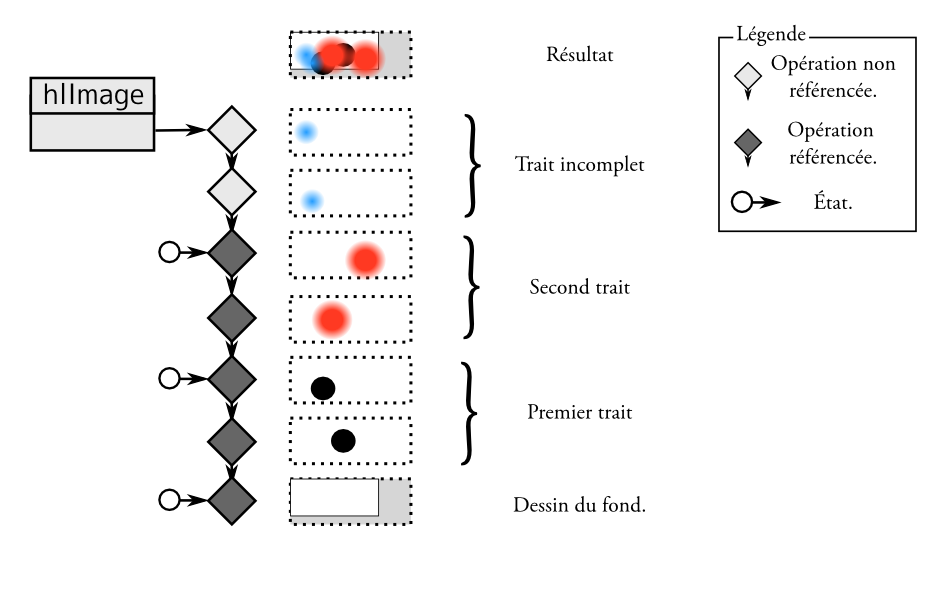
\includegraphics[width=\textwidth]{images/draw} 
			\label{fig:draw}
			\caption{Fonctionnement de la peinture}
		\end{figure}

			Ce mécanisme est résumé au schéma~\ref{fig:draw}, page~\ref{fig:draw}.
			
		\subsection{Undo/Redo}
			L'undo redo fonctionne de la manière décrite au chapitre précédent.
			Une pile maintient une liste des états de chaque traits, permettant de défaire
			et refaire les opérations. 

			Comme indiqué au chapitre précédent, la consommation de mémoire est de
			l'ordre du nombre d'états. Comme il n'y a pas de mécanisme permettant de
			réguler les caches de manière globale, nous limitons le nombre d'états disponibles
			à 16.
		\subsection{Visualisation}
			L'utilisateur visualise son dessin en temps réel via une fenêtre de visualisation.
			Celle-ci est décrite par sa taille en pixels, sa position sur le dessin, ainsi
			que son niveau d'échelle. 
			
			À chaque rafraichissement (entre 30 et 60 fois par secondes), les tiles correspondant
			à la région sont identifiés, rasterisés, et copiés dans le buffer correspondant à la région
			afin d'être visualisés. 

			Les rafraichissement se font indépendemment de l'ajout d'opérations. Un nombre quelconque
			d'opération peut donc avoir été ajouté entre deux rasterisations de l'image.

			L'utilisateur peut modifier la région de visualisation de trois manières différentes :

			\begin{itemize}
				\item Déplacer la région.
				\item Redimensionner la région.
				\item Changer l'échelle de visualisation.
			\end{itemize}

			Alors que déplacer et redimensionner la région ne demande que de recalculer les quelques tiles de la nouvelle
			bordure, changer l'échelle demande de recalculer l'entièreté de la région de visualisation. On peut
			donc s'attendre à ce que le déplacement et le redimensionnement de la région de visualisation soient 
			beaucoup plus rapides que le changement d'échelle.

	\section{Problématique}
		L'algorithme de rasterisation présenté jusqu'ici n'a aucune notion de localité d'opérations. Quelque soit le tile
		que nous voulons rasteriser, l'algorithme va appeler chacune des opérations. Si ces opérations ne s'appliquent pas
		au tile, celles-ci ne vont pas le modifier et vont donc s'exécuter très rapidement. Cependant, dans le cas de la 
		peinture, chaque tile n'est en réalité affecté que par un très petit pourcentage des opérations, et le nombre
		d'appel à ces opérations inutiles va en pratique ralentir de manière substentielle la rasterisation.

		Ce cas est particulièrement problématique lors du déplacement de la région de visualisation. Après avoir fait
		un large nombre de traits de peinture dans la région courante, l'utilisateur décide de déplacer la région de
		visualisation. De nouveaux tiles doivent donc être affichés. Pour ce faire l'algorithme de rasterisation va 
		examiner toutes les opérations des traits que l'utilisateur vient de faire, alors qu'aucun de ces traits n'affectent
		ces nouveaux tiles. 

		Il faut donc permettre à l'algorithme de rasterisation de pouvoir éviter d'examiner toute opération qui n'affecte
		pas les tiles. Au lieu d'avoir un algorithme de rasterisation en $O(n)$ ou $n$ est le nombre d'opérations
		ajoutées depuis le dernier rendu, nous aimerions avoir pour $n$ le nombre d'opérations ajoutées depuis le dernier
		rendu \emph{qui affectent le tile}.
		
		Deux approches ont été testées: Les opérations vectorisées, et Le saut d'opération.	


	\section{Bounding Boxes}
\newcommand{\BB}{\emph{BB}~}
		Une première étape est d'ajouter à toutes les opérations de dessin une \emph{Bounding Box} --- \BB en abrégé.
		Celle-ci représente
		Une région rectangulaire, alignée aux axes de l'image affectée par l'opération. Avant de rasteriser une opération 
		sur un tile, la \BB est examinée pour voir si le tile est affecté. s'il ne l'est pas, on peut éviter 
		de faire appel à la fonction de l'opération qui aurait de toute manière implémenté un tel mécanisme 
		de manière interne.

		Un autre intéret d'un tel système est que la \BB est générée à la création de l'opération, et non à
		chaque appel de l'opération, ce qui améliore encore les performances. TODO
		
		Pour réaliser cela, chaque classe d'opération doit donc être capable de générer de telles \BB.

		Si les \BB améliorent nettement les performances, elles n'améliorent pas la complexité
		temporelle de la rasterisation. Elles constituent cependant une base solide pour les deux solutions suivantes. 

	\section{Opérations vectorisées}
		\begin{figure}[ht]
			\centering
			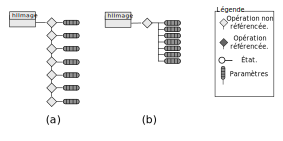
\includegraphics[width=\textwidth]{images/vector} 
			\label{fig:vector}
			\caption{(a) Opérations normales, (b) Opérations vectorisées}
		\end{figure}
		Vectoriser les opérations consiste à regrouper des opérations du même type en une seule opération qui contient
		un vecteur de paramètres représentant l'ensemble des paramètres. La \BB de l'opération
		vectorisée englobant les \BB des opérations qui la composent. Ceci est représenté au 
		schéma~\ref{fig:vector}, page~\pageref{fig:vector}
		Les opérations vectorielles ont plusieurs intérèts:
		\begin{itemize}
			\item La structure hlOperation est mise en commun, permettant d'économiser la mémoire.
			\item Si un paramètre des opérations est constant dans le vecteur, celui-ci peut être mis en commun,
			ce qui économise de la mémoire. Ceci arrive régulièrement en peinture; les traits sont principalement
			composés de brushes de même couleur et de même diamètre. \emph{brushes}
			\item Un test sur la Bounding box de l'opération vectorielle permet d'éviter le test de l'intégralité
			des opérations internes.
		\end{itemize}
		Mais ne sont pas sans limites:
		\begin{itemize}
			\item Il n'est pas possible de vectoriser des opérations de type différent. Ce système ne fonctionnerait
			donc pas pour un pinceau qui peindrait une alternance de cercles et de carrés.
			\item Il n'est pas possible de placer un état au milieu d'opérations vectorisées.
			\item L'algorithme de rasterisation doit être lourdement modifié pour pouvoir supporter ce type d'opérations.
			\item Les opérations vectorisées ne peuvent être modifiées avec l'API classique.
		\end{itemize}
		Les performances des opérations vectorisées seront donc contraintes par le nombre d'opérations du même type que
		l'on trouve entre chaque état. Pour l'application de peinture développée, les opérations sont toujours du même
		type, et un trait faisant en moyenne 100 opérations (TODO), le nombre de tests de bounding box à réaliser en 
		dehors des traits est divisé par 100. Le nombre de tests à réaliser sur les traits, augmente en contrepartie d'un
		pourcent.

		Nous n'atteignons donc pas notre objectif de réduction de complexité, mais les opérations vectorisées devraient
		augmenter en moyenne d'un facteur 100 le nombre d'opérations utilisables dans un document.

		\subsection{Impact sur l'API}
		Étant donné les limitations des opérations vectorisées, nous sommes obligés de donner à l'utilisateur un
		certain contrôle sur celles-ci. Nous proposons donc une fonction supplémentaire :
			\paragraph{\lstinline$void hlOpVectorise(hlOperation *op)$}
			\begin{description}
				\item[pre]: op est une opération qui n'est pas encore insérée dans la pile.
				\item[post]: op est une opération vectorisée. Toute opération non vectorisée du même
				type qu'op insérée sur la pile au dessus de op sera vectorisée dans op, jusqu'à ce
				que op soit sauvegardée dans un état.
			\end{description}
		Ainsi, l'utilisateur n'a qu'à utiliser cette fonction sur la première opération de chaque trait pour pouvoir
		vectoriser les traits. 
		\subsection{Évaluation des performances}

	\section{Bounding Operations}
\newcommand{\BO}{\emph{BO}~}
		\begin{figure}[ht]
			\centering
			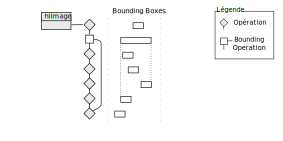
\includegraphics[width=\textwidth]{images/bo} 
			\label{fig:bo}
			\caption{Une Bounding Operation}
		\end{figure}
		Les \emph{Bounding Operations} -- \BO en abrégé --- ne sont pas des opérations au sens original du terme puisque si utilisées
		correctement, elles n'effectuent aucune modification de l'image. Cependant elles s'utilisent et s'insèrent
		dans la pile comme des opérations classiques d'une nouvelle catégorie. 
		
		Les \BO contiennent une \BB et une référence vers une opération antérieure.
		La rasterisation des \emph{Bounding Opérations} fonctionne de la manière suivante:
		\begin{itemize}
			\item Rasteriser un tile à l'intérieur de la \BB consiste à rasteriser l'opération précédente.
			\item Rasteriser un tile à l'extérieur de la \BB consiste à rasteriser l'opération antérieure référencée.
		\end{itemize}

		En créant une \BO dont la \BB englobe les \BB d'une suite
		d'opérations qui la précedent, et en faisant pointer la \BO sur une opération précédant 
		cette suite, on permet à l'algorithme de rasterisation de contourner la suite d'opérations.
		
		Ce principe est représenté au schéma~\ref{fig:bo}, page~\pageref{fig:bo}

		Les \BO ne modifiant pas l'apparence de l'image, on peut les placer où l'on veut dans la pile. Ces 
		opérations peuvent donc "enjamber" des états, permettant des groupements qui ne sont pas possibles avec les opérations
		vectorisées.

		\begin{figure}[ht]
			\centering
			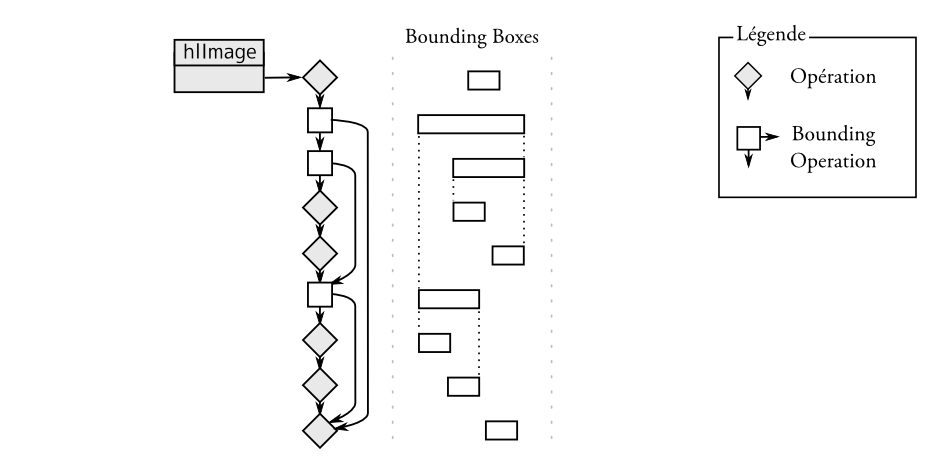
\includegraphics[width=\textwidth]{images/bo2} 
			\label{fig:bo2}
			\caption{Une Bounding Operation Hierarchy}
		\end{figure}

		Là où les \BO deviennent très intéressantes c'est qu'on peut les emboiter les unes dans les
		autres de manière récursive, et ainsi offrir une structure semblable à une \emph{Bounding Volume Hierarchy} 
		--- \emph{BVH} en abrégé --- ou à des \emph{KD-Trees}. On appelle \emph{Bounding Operation Hierarchy} --- \emph{BOH}
		en abrégé --- ce type de structures. Lorsque les \BO ne s'imbriquent pas, on appelle la structure \emph{Bounding Object Sequence},
		--- \emph{BOS} en abrégé. Un exemple de \emph{BOH} est représenté au schéma~\ref{fig:bo2}, pageref~\pageref{fig:bo2} 

		\begin{figure}[ht]
			\centering
			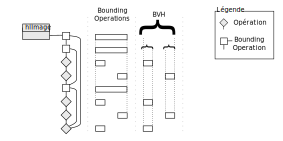
\includegraphics[width=\textwidth]{images/bo3} 
			\label{fig:bo3}
			\caption{Cas critique pour les \emph{BOH}}
		\end{figure}
		Il y a cependant une grande différence entre les \emph{BVH}, et les \emph{BOH}; là où un \emph{Bounding Volume}
		peut contenir n'importe quel ensemble
		d'objets dans la scène, une \BO ne peut contenir que des opérations qui se suivent temporellement. Il
		est très simple de construire un exemple ou les \emph{BVH} excellent et les \emph{BOH} ne font qu'empirer
		les choses, comme sur le schéma~\ref{fig:bo3}, page~\pageref{fig:bo3}. Heureusement de tels cas arrivent peu 
		en pratique, puisque les outils de peinture tendent à grouper les opérations.

		Il serait cependant possible d'approcher l'efficacité d'un \emph{BVH} en procédant à un réordonancement intelligent
		des opérations. 
		
		Une autre différence de taille est que les \emph{BVH} sont conçus pour organiser des scènes statiques,
		et non pour des scènes pouvant changer selon les états. Ces différences nous empèchent de reprendre 
		les algorithmes développés pour les \emph{BVH} et les \emph{KD-Trees}, 
		même si nous pouvons en reprendre les idées et les principes. 

		Une première tâche intéressante consiste à construire la \emph{BOH}. La littérature sur les \emph{BVH}
		décrit deux types d'algorithmes:
		\begin{description}
			\item[Algorithmes Inline] Ces algorithmes construisent la \emph{BVH} au fur et à mesure
			que l'on ajoute des objets dans la scène --- des opérations dans l'image. Ces algorithmes 
			semblent donc particulièrement adaptés à la peinture puisqu'ils fonctionneront au fur et à mesure que l'utilisateur
			peint. Ces algorithmes 
			\item[Algorithmes Offline] Ces algorithmes construisent la \emph{BVH} à partir d'une 
			scène déjà construite --- d'un pile d'opération existante. Ces algorithmes ont l'avantage de pouvoir
			créer des hiérarchies optimales (selon différents critères). Le problème est qu'ils prennent un certain temps 
			à s'exécuter, ce qui n'est pas idéal pour un framework dédié à l'édition interactive. 
		\end{description}
		Seul des algorithmes inline ont pour l'instant été explorés et implémentés. Un algorithme crée des \emph{BOS} ,
		et l'autre des \emph{BOH}. 
		
		\subsection{Bounding Operation Sequence}
			Le premier algorithme testé et implémenté est un algorithme créant une suite de \BO plutôt
			qu'une hiérarchie.
			
			\subsubsection{Placement des \BO dans la pile}
			Le placement des \BO dans la pile fonctionne de la manière suivante: Initialement, la \BO possède une \BB
			de taille nulle, et est dans l'état dit \emph{ouvert} Lorsque l'on insère cette \BO au dessus de la pile, 
			celle-ci prend pour comme opération de référence l'opération précédente. 

			Lorsque l'on insère une opération sur la pile, au dessus d'une \BO ouverte, la \BB de la \BO est étendue
			pour englober la \BB de la nouvelle opération. La \BB est ensuite repositionnée au dessus de la pile. 

			L'on peut continuer à insérer des opérations de cette manière jusqu'à ce que la \BO soit \emph{fermée},
			auquel cas elle se comporte comme une opération normale. 

			\subsubsection{Fermer les \emph{Bounding Operations}}
			Ce premier algorithme va donc ajouter des \BO ouvertes, les fermer au moment opportun et puis directement 
			en rajouter une nouvelle ouverte. La question est donc quand fermer les \BO. Il s'agit ici plus
			de trouver une bonne heuristique que d'établir une stratégie optimale. Il y a plusieurs critères de clotures
			que nous pouvons combiner:

			\begin{description}
				\item[Rapport de surface des \BB]. Nous comparons ici le rapport entre la surface de
				la \BB de la \BO, et la surface couverte par l'union de \BB des opérations contenues. Plus ce rapport
				est grand, moins la \BB de la \BO correspond bien à la surface couverte par les opérations, et donc
				moins elle est efficace. Un rapport maximal peut donc être envisagé comme critère de cloture.
				\item[Nombre d'opérations dans \BO]. Au plus la \BO contient d'opérations,
				Au moins d'opérations devront être examinées en dehors de la BB de celle-ci, mais au plus il
				faudra en tester à l'intérieur de celle-ci. Un compromis optimal est difficile à trouver puisque
				celui-ci dépend de l'échelle de visualisation. 

				\item[Sauvegarde d'un état] Bien que les \BO sont capable d'englober des états, la sauvegarde
				d'un état marque la cloture d'un trait et donc une grande probabilité de discontinuité dans
				le placement des opérations. 
			\end{description}
			Différentes heuristiques basées sur ces critères ont été testées : /TODO resultat des perfs.

		\subsection{Bounding Operation Hierarchy}
			Cet algorithme permet de créer une hiérarchie de \BO d'une profondeur fixe. Dans cet algorithme chaque niveau
			fonctionne exactement comme l'algorithme précédent en considérant les \BO des opérations d'en dessous comme
			des opérations classiques. Chaque niveau pouvant avoir une heuristique séparée. 

		\subsection{Impact sur l'API}
			Les \BO ont un impact minimal sur l'API. Il suffit d'ajouter une opération de type \BO avec les paramètres
			appropriés pour que les mécanismes se mettent en place. Une fois en place les \BO n'influent quasiment pas
			sur les actions que l'on peut réaliser sur une hlImage. 

			Par contre, le fait que les \BO puissent être déplacées automatiquement par d'autres opérations perturbe
			l'accès aux opérations par indice. Pour résoudre ce problème, les \BO sont ignorées lors des accès par
			indice. 

			Si l'algorithme de rasterisation ne doit pas être grandement modifié, les algorithmes de modification
			de la pile doivent être revus pour préserver la cohérence des BVH.

			\subsubsection{Forking}
			\begin{figure}[ht]
				\centering
				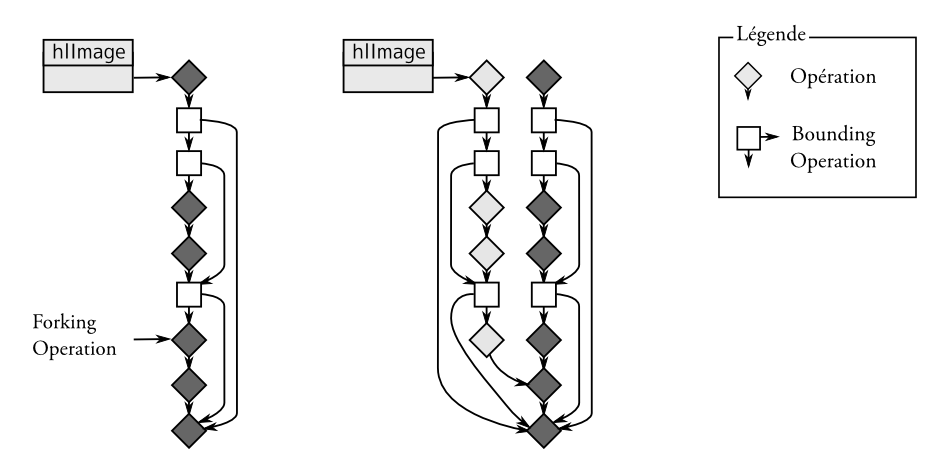
\includegraphics[width=\textwidth]{images/bo-forking} 
				\label{fig:bo-forking}
				\caption{Forker des \BO}
			\end{figure}
			L'opération de forking doit duplique également les \BO. Le schéma~\ref{fig:bo-forking}, page~\pageref{fig:bo-forking} montre une pile
			contenant des \BO avant et après forking. 

			La difficulté réside donc à réassocier les références correctement. 
			Ceci se fait en reprenant l'algorithme de forking en applicant les modifications suivantes:
			\begin{itemize}
				\item Lorsque l'on duplique une \BO, son duplicata continue à pointer vers l'opération originale.
				On associe ensuite dans une Hashtable l'uid de l'opération pointée
				par la \BO à cette \BO. 
				\item Lorsque l'on duplique une opération (\BO comprise), on regarde si son uid est présente dans
				la HashTable. Dans l'affirmative, la \BO correspondante pointe désormais sur cette opération, et
				l'uid est retiré de la HashTable.
			\end{itemize}
			L'opération de forking garde donc toujours la même complexité temporelle, mais gagne une complexité spatiale
			de $O(n)$ où $n$ est la profondeur maximale de la \emph{BOH}, la profondeur des \emph{BOH} étant en $O(log(n))$, où $n$
			est le nombre total d'opérations dans la pile. 
			
			\subsubsection{Retrait d'opérations}
			\begin{figure}[ht]
				\centering
				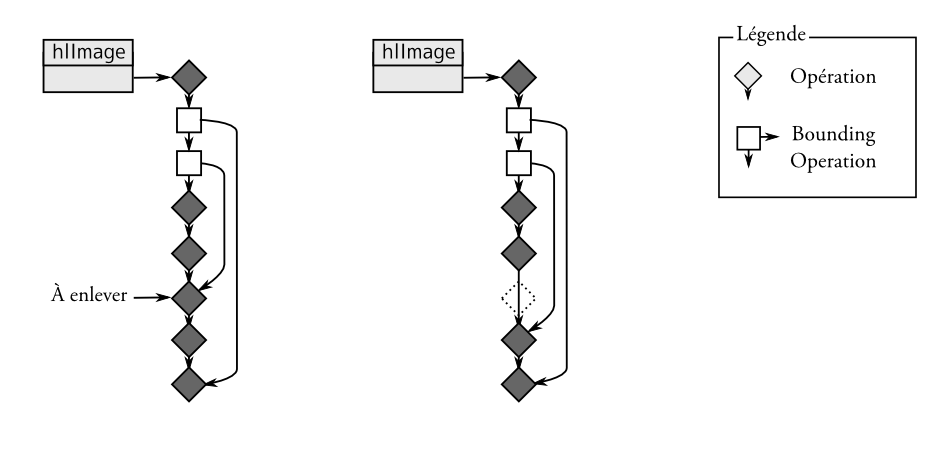
\includegraphics[width=\textwidth]{images/bo-supress} 
				\label{fig:bo-supress}
				\caption{Retirer une opération pointée par une \BO}
			\end{figure}
			Le retrait d'une opération dans la pile peut être problématique si un \BO pointe sur cette opération. Dans de
			tel cas, il faut détecter les \BO qui pointent et les faire pointer vers l'opération précédente à celle
			que l'on veut retirer. Si il n'y a pas de telle opération précédente, il faut remplacer l'opération à retirer
			par une opération qui ne fait rien. Il faut également supprimer les \BO qui ne contiennent d'opération autre
			que des \BO.  Un exemple de retrait d'opération dans une pile contenant des \BO est représenté au 
			schéma~\ref{fig:bo-supress}, page~\pageref{fig:bo-supress}
			
			Ceci ne modifie pas la complexité temporelle, mais ajoute une complexité spatiale
			de $O(n)$ ou $n$ est le nombre de \BO pointant l'opération à retirer. Ce nombre est également borné par
			la profondeur de la \emph{BOH}, ce qui ramène cette complexité à $O(log(n))$ ou $n$ est le nombre d'opérations dans
			la pile jusqu'à l'opération à retirer. 

			\subsubsection{Insertion et Modification d'opérations}
			\begin{figure}[ht]
				\centering
				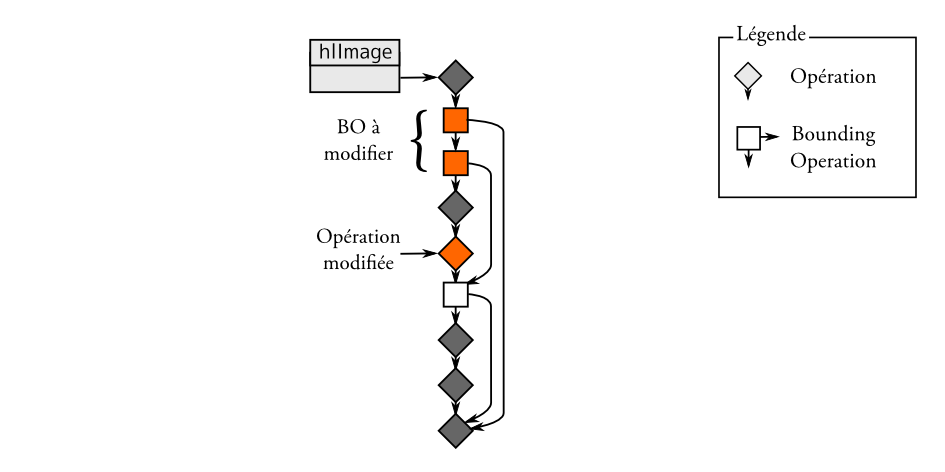
\includegraphics[width=\textwidth]{images/bo-modify} 
				\label{fig:bo-modify}
				\caption{Modifier une opération dans une pile contenant des \BO}
			\end{figure}
			Insérer ou modifier des opérations peut invalider les \BB des \BO qui englobent ces opérations. Il faut
			donc détecter ces \BO, et modifier leur \BB afin qu'elles contiennent la \BB de l'opération à insérer, ou la
			nouvelle \BB de l'opération modifiée, ce qui se fait en parcourant la pile jusqu'à l'emplacement d'insertion,
			ou jusqu'à l'opération à modifier de la manière suivante
			\begin{itemize}
				\item Lorsque l'on rencontre une \BO, on l'associe dans une Hashtable à l'opération pointée.
				\item Lorsque l'on rencontre une opération, on retire la \BO associée dans la Hashtable.
				\item Lorsque l'on arrive à l'emplacement voulu, ou à l'opération à modifier, la Hashtable
				contient la liste des \BO à modifier.
			\end{itemize}
			Cela ne modifie donc pas la complexité temporelle, mais ajoute une complexité spatiale, en $O(log(n))$ où $n$
			est le nombre d'opérations dans la pile.

		\subsection{Évaluation des performances}
			Pour évaluer les performances, nous avons enregistré les étapes de création de plusieurs dessins, chacun d'entre eux representant
			un cas d'utilisation différent. Ces dessins de taille variable ont été réalisés sur une feuille de $4.8*10^17$ pixels. Nous avons 
			ensuite rejoué ces étapes (ajout d'opérations, rasterisation, zoom, dézoom, undo, redo,
			déplacement du viewport) en ommettant les pauses afin de mesurer le temps total pris par le framework pour dessiner le dessin.

			\begin{figure}[h]
				\centering
				\captionsetup[subfigure]{labelformat=empty}
				\subfloat[$(a)$~Dessin technique, 25Mpixels]{ 
\includegraphics[width=0.5\textwidth]{images/tests/test_a} }
				\subfloat[$(b)$~Hachures, $0.5$Gpixels]{ \label{fig:testb} 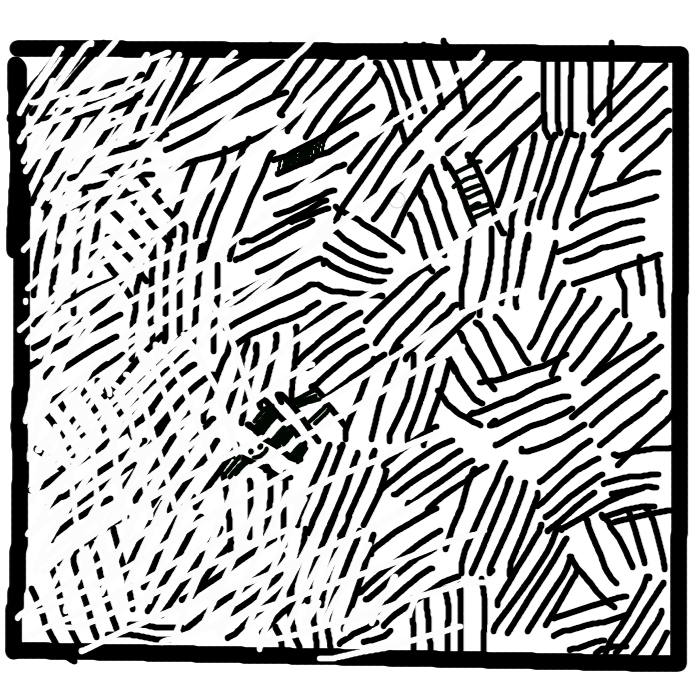
\includegraphics[width=0.5\textwidth]{images/tests/test_b} }
				\\
				\subfloat[$(c)$~Portrait, $25$Mpixels]{ \label{fig:testc} 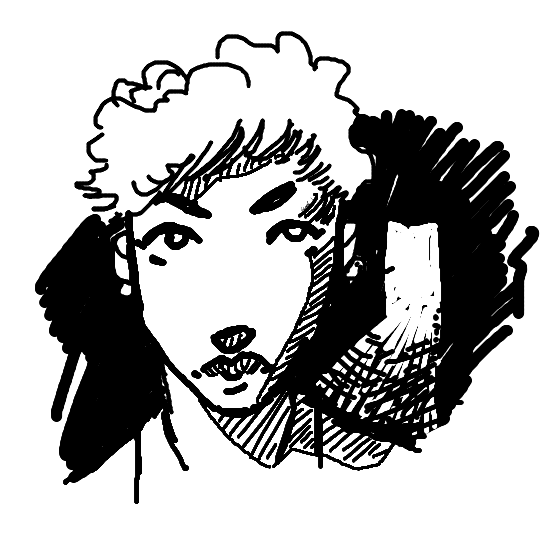
\includegraphics[width=0.5\textwidth]{images/tests/test_c} }
				\subfloat[$(e)$~Test divers, $0.5$Gpixels]{ \label{fig:testc} 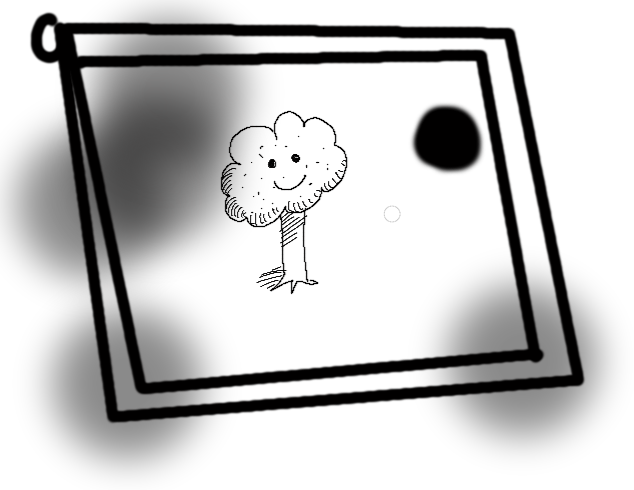
\includegraphics[width=0.5\textwidth]{images/tests/test_e} }
				\\
				\subfloat[$(d)$~Paysage avec petits détails, $2$Gpixels]{ \label{fig:testd} 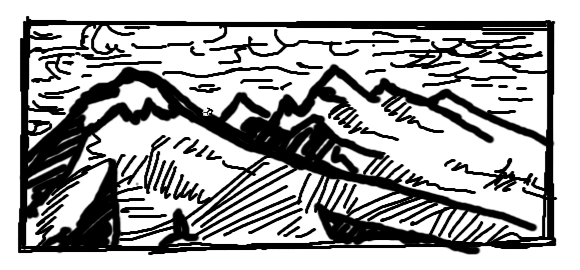
\includegraphics[width=\textwidth]{images/tests/test_d} }
				\label{fig:testdrawings}
				\caption{Dessins utilisés pour les tests de performances}
			\end{figure}

			Les cinq dessins sont présentés à la figure~\ref{fig:testdrawings}, page~\pageref{fig:testdrawings}

			\subsubsection{Taille des \BO}
				Le premier test utilise une heuristique qui ferme la boite quand celle-ci contient un certain nombre d'opérations, ou
				quand un nouvel état est enregistré.

				\begin{table*}
					\tiny
					\label{boxdepth}
					\begin{tabular*}{\textwidth}{@{\extracolsep{\fill}} | c || c | c | c | c | c | c | c | c | c | c |}
						\hline
						& \multicolumn{10}{c|}{Nombre maximal d'opérations par \BO} \\
						\hline
								&8		&  16		&  32		&  64		&  128		&  256		&  512		&  1024		&  2048		&  4092		 \\
						\hline
						\hline
						Dessin & \multicolumn{10}{c|}{Temps de calcul (sec)} \\
						\hline
						 A		& 249.67	&  117.81	&  72.01	&  52.00	&  39.13	&  34.32	&  32.87	&  32.84	&  32.99	&  32.83	 \\
						 B 		& 847.67	&  312.65	&  113.12	&  70.14	&  52.35	&  40.44	&  39.45	&  41.32	&  42.51	&  42.78	 \\
						 C		& 1283.64	&  550.17	&  354.88	&  154.36	&  138.46	&  163.26	&  104.11	&  94.40	&  108.18	&  146.60	 \\
						 D		& 1181.11	&  466.45	&  278.11	&  144.25	&  170.93	&  132.44	&  91.03	&  89.84	&  88.35	&  140.39	 \\
						 E		& 61.32		&  38.71	&  18.21	&  12.93	&  11.81	&  11.19	&  11.01	&  11.08	&  10.72	&  11.15	 \\
						\hline
					\end{tabular*}
				\end{table*}
				\begin{figure}[h]
					\centering
					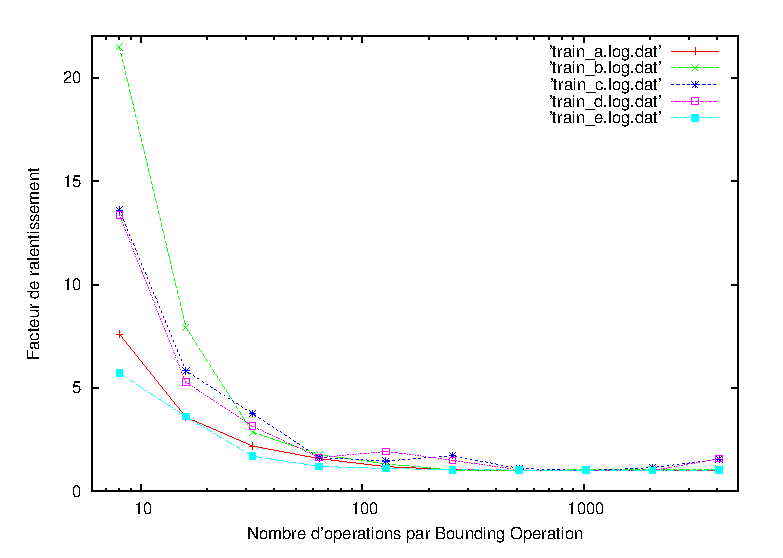
\includegraphics[width=\textwidth]{images/depthgraph.eps} 
					\label{fig:depthgraph}
				\end{figure}
				
				Le tableau ... évalue l'influence du nombre d'opérations par \BO sur la fluidité du programme. 

				\begin{table*}
					\tiny
					\label{boxratio}
					\begin{tabular*}{\textwidth}{@{\extracolsep{\fill}} | c || c | c | c | c | c | c | c | c |}
						\hline
						& \multicolumn{8}{c|}{Aire maximale accumulée par \BO} \\
						\hline
								& 2		& 4		& 8		&  16		&  32		&  64		&  128		&  512		\\
						\hline
						\hline
						Dessin & \multicolumn{8}{c|}{Temps de calcul (sec)} \\
						\hline
						D		& 656.04	&  358.37	&  158.52	&  153.24	&  159.39	&  149.18	&  148.01	&  98.38	\\
						A		& 70.85		&  51.89	&  41.54	&  37.51	&  35.72	&  34.89	&  36.23	&  54.46	\\
						B		& 225.32	&  139.10	&  100.74	&  83.29	&  45.69	&  42.70	&  41.45	&  43.58	\\
						E		& 16.21		&  12.59	&  11.73	&  12.30	&  11.44	&  10.62	&  11.13	&  10.66	\\
						C		& 585.40	&  321.23	&  141.87	&  163.36	&  156.43	&  145.06	&  143.24	&  141.66	\\
						\hline
					\end{tabular*}
				\end{table*}
				\begin{figure}[h]
					\centering
					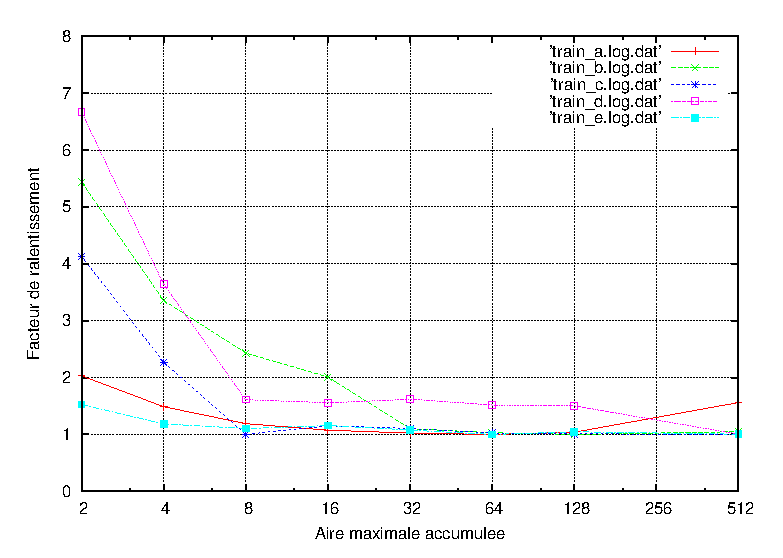
\includegraphics[width=\textwidth]{images/graph_ratio.eps} 
					\label{fig:depthgraph}
				\end{figure}

				\begin{table*}
					\tiny
					\label{boxdepth1}
					\begin{tabular*}{\textwidth}{@{\extracolsep{\fill}} | c || c | c | c | c | c | c | c | c | c | c |}
						\hline
						& \multicolumn{10}{c|}{Nombre maximal d'opérations par \BO} \\
						\hline
								&8		&  16		&  32		&  64		&  128		&  256		&  512		&  1024		&  2048		&  4092		 \\
						\hline
						\hline
						Dessin & \multicolumn{10}{c|}{Temps de calcul (sec)} \\
						\hline
						A		& 56.33		&  35.43	&  33.72	&  33.41	&  33.57	&  33.32	&  32.82	&  34.31	&  34.76	&  34.26	\\
						B		& 53.30		&  70.24	&  67.47	&  66.61	&  64.70	&  41.40	&  42.01	&  43.41	&  44.54	&  44.36	\\
						C 		& 107.27	&  144.32	&  141.42	&  94.17	&  91.31	&  123.96	&  142.79	&  141.63	&  142.71	&  148.53	\\
						D		& 144.20	&  88.20	&  86.48	&  115.26	&  140.11	&  147.81	&  141.73	&  101.48	&  88.51	&  108.78	\\
						E		& 17.88		&  17.06	&  16.89	&  16.67	&  16.32	&  16.59	&  16.51	&  16.59	&  16.88	&  16.28	\\
						\hline
					\end{tabular*}
				\end{table*}
				\begin{figure}[h]
					\centering
					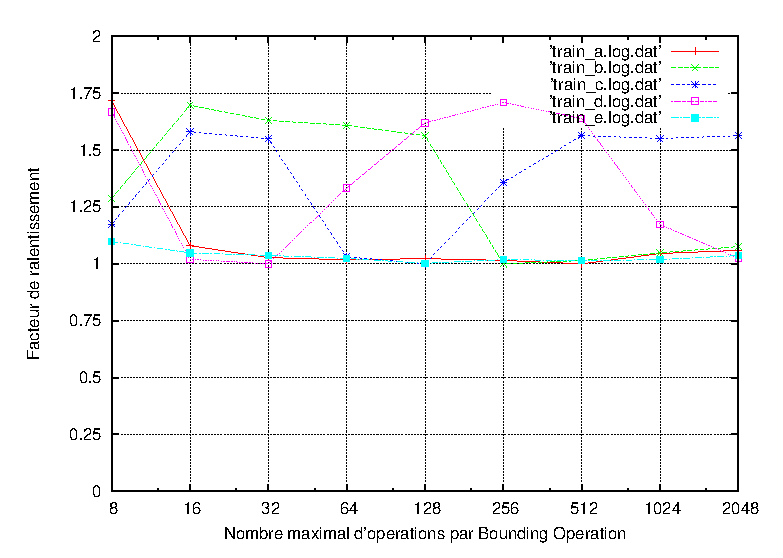
\includegraphics[width=\textwidth]{images/depthgraphd1.eps} 
					\label{fig:depthgraphd1}
				\end{figure}

				\begin{table*}
					\tiny
					\label{boxdepthr1}
					\begin{tabular*}{\textwidth}{@{\extracolsep{\fill}} | c || c | c | c | c | c | c | c | c | }
						\hline
						Dessin & \multicolumn{8}{c|}{Temps de calcul (sec)} \\
						\hline
						\BO Internes 	& \multicolumn{4}{c|}{32}					&  \multicolumn{4}{c|}{64}	\\					
						\hline
						\BO Externes	& 4		&  8		&  16		&  32		&  4		&  8		&  16		&  32		       \\
						\hline
						A		& 45.88		&  37.45	&  34.88	&  33.09	&  37.64	&  33.91	&  32.77	&  33.04	       \\
						B 		& 100.87	&  47.39	&  43.65	&  43.07	&  49.19	&  43.15	&  42.85	&  41.30	       \\
						C 		& 127.49	&  137.28	&  142.36	&  136.36	&  103.51	&  108.55	&  140.65	&  140.19		\\
						D		& 193.25	&  153.72	&  142.94	&  140.80	&  156.07	&  145.47	&  139.30	&  134.22		\\
						E		& 19.08		&  17.22	&  17.02	&  16.51	&  17.87	&  16.68	&  14.64	&  11.18	       \\
						\hline
						\BO Internes 	&  \multicolumn{4}{c|}{128}					& \multicolumn{4}{c|}{256}   \\
						\hline
						\BO Externes	&  4 		&  8		&  16		&  32		&  4		&  8		& 16		&  32		\\
						\hline
						A		&  35.29	&  33.64	&  50.20	&  54.35	&  53.44	&  54.52	&  57.16	&  55.31	\\
						B 		&  43.39	&  50.90	&  63.60	&  63.78	&  65.60	&  66.61	&  46.07	&  42.05	\\
						C 		&  142.59	&  136.45	&  138.14	&  138.23	&  139.82	&  97.75	&  88.15	&  138.16	\\
						D		&  139.39	&  141.59	&  91.14	&  88.86	&  137.26	&  137.37	&  137.34	&  137.08	\\
						E		&  12.81	&  11.17	&  10.95	&  10.66	&  11.02	&  11.07	&  10.75	&  10.56	\\
						\hline
					\end{tabular*}
				\end{table*}
				\begin{figure}[h]
					\centering
					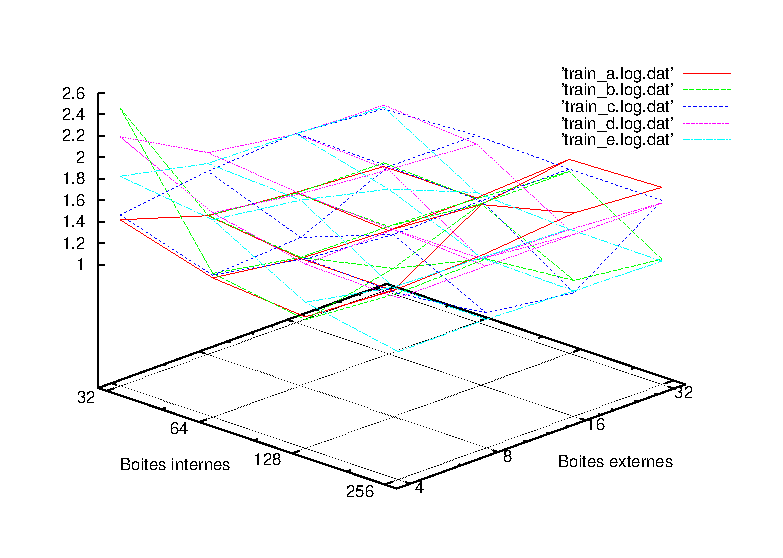
\includegraphics[width=\textwidth]{images/depthgraphr1.eps} 
					\label{fig:depthgraphr1}
				\end{figure}




\chapter{Anti-aliasing (15 pages) }
	\section{Primitive de dessin}
	\section{Problèmes d'échelle}
		\subsection{Oversampling}
	\section{Problèmes de superposition}
	\section{Problèmes de bandes}
	\section{Problème de blending à faible opacité}
	\section{Problème de précision de positionement}
\chapter{Test utilisateurs (10 pages) }
	\section{Procédure}
	\section{Résultats}
	\section{Analyse}
\chapter{Comparaison d'Himalaya aux autres frameworks}
\chapter{Conclusion}
